

Finite elements models are widely used to estimate sodt tissue deformations under predefined boundary conditions. Several biomechanical models of the breast were recently developed providing physics-based predictions of tissue motion and internal stress and strain intensity. A biomechanical model obtained from patient's MRI volumes can be subsequently used to mimic breast compression during mammography acquisitions.\\


This chapter provides theoretical background on continuous mechanic theory applied to soft tissue modeling. The principles of finite element theory are described including solid bodies and contact mechanics. A review of the existing biomechanical breast models is given, presenting the main challenges in the field and the proposed solutions. These developments provide the core foundation of our proposed  patient specific breast model. 
      
\clearpage
\section{Continuous mechanics}
\label{section:continuousmechanics}
Continuous mechanics is a branch of mechanics that deals with the analysis of the kinematics and the mechanical behavior of materials modeled as a continuous mass. Continuous mechanics is based on the following hypothesis: the matter is continuously distributed throughout the space occupied by the matter. Its formulation relays on how physical quantities, as for example pressure, temperature, and velocity, are measured macroscopically.

In this section the continuous mechanis theory applied to solid bodies is described using the books by Belytschko T. et al. \citep{belytschko_nonlinear_2013} and Abeyaratne R. \citep{abeyaratne_continuum_2012}.
\subsection{Deformation and strain}\label{subsection:defromationandstrain}
Continuous mechanics is the mathematical description of how physical objects respond to the application of forces.

	A \textbf{body} is the mathematical abstraction of an \textbf{object} and is defined by its geometric and constitutive properties.  At a macroscopic level, a solid object is described as a homogeneous and continuous body. Then, the substance of the object has a unique composition and completely fills the space it occupies, ignoring the granular (atomic) nature of matter. In continuous mechanics, a body $\mathcal{B}$\nomenclature{$\mathcal{B}$}{Body} is composed of \textbf{particles} $p$ \nomenclature{$p$}{Particle or material point} (or material points). Each particle is located at some defined \textbf{point}  $x$ in three dimensional space. All the points corresponding to the locations of all the particles, constitute the \textbf{domain} $\Omega$ \nomenclature{$\Omega$}{Domain occupied by the body} occupied by the body in a given configuration, also named $geometry$. A particular body can change its configuration and therefore the occupied region in the space when exposed to some external stimulus, such as force, pressure or heat.
	
 The \textbf{configuration} of a body is defined as a one-to-one mapping between the particle $p$ and position $x$, $\Omega_0 = \chi_0 (\mathcal{B})$ (see figure \ref{reference_config_theory}). To describe the solid's response to external stimuli, one needs to know the changes in geometrical characteristics between at least two configurations: the configuration $\Omega_1$ that one wishes to analyze  \nomenclature{$\Omega_1$}{Current or analyzed body configuration }, and the \textbf{reference configuration} $\Omega_0$  relative to which the changes are to be measured\nomenclature{$\Omega_0$}{Reference body configuration }. Here, (Figure \ref{reference_config_theory}), the mappings $\chi_0$ and $\chi_1$ take $p \rightarrow X$\nomenclature{$X$}{Point position on the reference configuration} and $p \rightarrow x$\nomenclature{$x$}{Point position on the current configuration}, where $X$ and $x$ are the positions of particle $p$ in the two configurations under consideration.

Frequently, the reference configuration is fixed for a given study and is arbitrarily chosen in a the most convenient way among all the configurations that the body can sustain. 
 
 The \textbf{deformation} of the body from the reference configuration $\Omega_0$ is characterized by the next defined mapping $\Phi$:
 \begin{equation} 
 x = \Phi(X) = \chi_1(\chi_0^{-1}(X)), \ \ \  where \ \  X \in \Omega_0 \ and \ x \in \Omega_1
 \label{referenceToCurrentCoordinates}
 \end{equation}
 
 The \textbf{displacement} $u$\nomenclature{$u$}{Particle displacement} of a particle is the difference between its position in the analyzed configuration (or current configuration) and its position in the reference configuration.
 \begin{equation}
 u(X) = \Phi(X) - X
 \end{equation}


\begin{figure}
\begin{center}
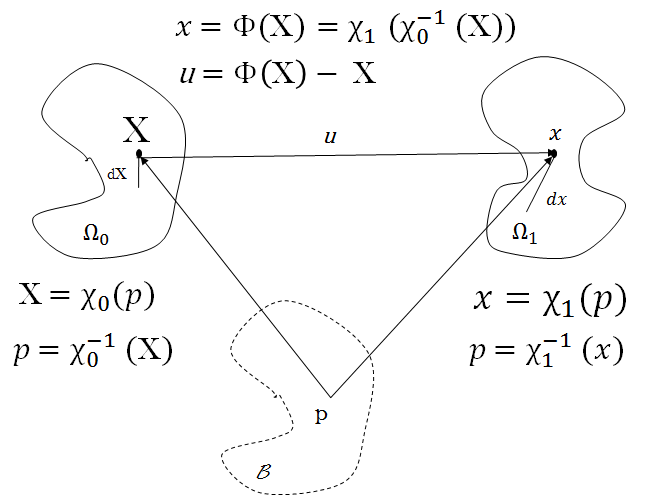
\includegraphics[width=0.7\textwidth,keepaspectratio]{figures/referenceFig.png} 
\caption{ The position of a particle in the reference and current body configurations.}
\label{reference_config_theory}
\end{center}
\end{figure}

Suppose that $G(\Omega_1)$ is the value of some extensive physical property  associated with the body $\mathcal{B}$ in the current configuration (such as the body mass $m$\nomenclature{$m$}{Body mass}). It exists a density $g(x)$ such that:
\begin{equation}
 G(\Omega_1) = \int_{\Omega_1} g(x)dv
\end{equation} 

 where $dv$ is the volume of the material element.
 Thus, the property $G(\Omega_1)$ is related to the body, while the density $g(x)$ is related to the position of the body particle.
\subsubsection*{Eulerian and Lagrangian formulations}
There are two classical techniques used to describe the body physical characteristics depending on the choice of independent variables.
 Some physical characteristics, such as the mass density, can be defined for each individual particle. In such a case, the body characteristics are defined by: 
\begin{equation}
\forall	p \in \mathcal{B}, \ m = \mathcal{M}(p).
\end{equation} 

Here the coordinate system remains consistent and moves with the particle. Therefore, the coordinates of both the particle and the attached variable do not change along the deformation. A particle is an abstract entity and cannot be used in numerical calculations. Therefore, it is described by its location in the reference configuration $p= \chi_0^{-1}(X)$ .
\begin{equation}
 m =  \mathcal{M}(p) = \mathcal{M}(\chi_0^{-1}(X))
\end{equation}

 We call $X$ Lagrangian or material coordinates, and its application is called Lagrangian or material description.  
 

Instead of defining body characteristics as a function of body particles, one can define directly a body as a function of particle locations in current configuration by using the relation $ x = \chi_1(p)$, and therefore 
\begin{equation}
m = \tilde{ \mathcal{M}}(x) = \mathcal{M}(\chi_1^{-1}(x))
\end{equation}

 Here the coordinate system is fixed and the particle coordinates are changing. Therefore, the position of particles, and any related quantity, change during the deformation. We call $x$ Eulerian or spatial coordinates, and its application is called Eulerian or spatial description.
 
 These approaches are distinguished by three important aspects: the mesh description, the stress tensor and momentum equilibrium, and the strain measure. The advantages and drawbacks of these two formulations will be discussed later in this chapter. Further, only Lagrangian formulation is used to describe the continuous deformation of soft tissue.       

\subsubsection*{Deformation gradient}\label{deformatiogradient}

In mathematical formulation the deformation gradient tensor $F$\nomenclature{$F$}{Deformation gradient} is the Jacobian matrix of the deformation $\Phi(X)$:
\begin{equation}
F = \frac{\partial \Phi (X)}{\partial X} = \frac{\partial x}{\partial X}
\end{equation}

Considering infinitesimal quantities, the deformation gradient relates the segment $dX$ in the reference configuration to the corresponding deformed segment $dx$ in the current configuration (Figure \ref{reference_config_theory}) 
\begin{equation}
dx = F \cdot dX.
\label{deformationGradRelation}
\end{equation}

In addition to the mapping of such vectors, the deformation gradient tensor allows also the mapping of differential volumes as:
\begin{equation}
dv = det(F)dV = JdV
\label{JacobianRelation}
\end{equation}

The Jacobian determinant $J$\nomenclature{$J$}{Jacobian determinant of the deformation gradient tensor} of the deformation gradient tensor $F$ is a measure of the volume variation during the deformation. It can be used to relate extensive physical properties in the current and reference configurations:

\begin{equation}
\int_{\Omega_1}g(x)dv = \int_{\Omega_0}g(\Phi(X))JdV
\end{equation}

\subsubsection*{Local decomposition of the deformation gradient tensor into rotation and stretch}\label{deformationgradienttensor}
The deformation gradient tensor $F$ completely characterizes
the body deformation in the vicinity of a particle p. This deformation consists, locally, of a rigid body rotation and a body \textit{stretch} (see Figure \ref{deformationGradientDecom}). As $dX$ and $dx$ are differential segments, the map $F$ is not affected by rigid-body translations.  

\begin{figure}
\centering
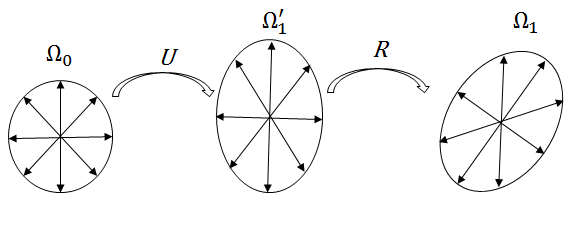
\includegraphics[width=0.7\textwidth,keepaspectratio]{figures/deformationTensorDecomposition.png} 
\caption[]{Local decomposition of the deformation tensor into stretch and rotation.  }
\label{deformationGradientDecom}
\end{figure}

Generally, the body stretch is defined as the ratio of the deformed line elements to the length of the corresponding undeformed line element \nomenclature{$l$}{Body stretch}
\begin{equation}
l = \frac{\vert dx \vert}{\vert dX \vert},
\end{equation} 
and consists locally on three mutually orthogonal stretches named \textbf{the principal stretches}.

According to the polar decomposition theorem, the deformation tensor can be written as the product of a proper orthogonal tensor $R$ representing the rotational part, and a symmetric positive defined tensor $U$ representing the body distortions 
\begin{equation}
F = R \cdot U.
\end{equation}
Where $U$ and $R$ are given by the relations $U = (F^T \cdot F)^ {\frac{1}{2}} $ and $R = F \cdot U^{-1}$. The essential property of tensor $U$ is that it is symmetric and positive, therefore it has three real positive eigenvalues
$\lambda_1, \lambda_2, \lambda_3$ and a corresponding triplet of orthonormal eigenvectors $r_1, r_2, r_3$. Thus, when an infinitesimal segment $dx$ is stretched by the tensor $U$, the segment is distorted in the principal directions of U by amounts of corresponding eigenvalues of U. The tensor $U$ is also called the \textbf{right stretch tensor}.  Since there is a one-to-one relation between $U$ and $U^2$, for the simplification of numerical calculus, the stretch tensor can by replaced by the \textbf{Green deformation tensor} $C = F^T \cdot F$.



There are three particular functions of $C$ called the principal invariants. 

\begin{equation}
\label{principal_invariants}
I_1(C) = tr C, \ \ I_2(C)=\frac{1}{2}\left[ trC^2 - \left(tr C \right)^2 \right], \ \ I_3(C)=det(C) .
\end{equation} 

These functions are related to the three principal stretches by the following relations:
\begin{equation}
\label{principalstrechinvariantsrelation}
I_1(C) = \lambda_1^2+\lambda_2^2+\lambda_3^2, \ \ I_2(C) = \lambda_1^2 \lambda_2^2 + \lambda_2^2 \lambda_3^2+ \lambda_3^2 \lambda_1^2, \ \ I_3(C) = \lambda_1^2 \lambda_2^2 \lambda_3^2
\end{equation}

The essential property of the principal invariants is that they do not change under coordinate transformations for a given body configuration. Their use to compute the body stretch is an essential part of constitutive modeling, because the behavior of a material should not depend on the coordinate system.

It also can be shown that:
\begin{equation}
\label{eq:detinvariantrelation}
det(C-\mu I) = -\mu ^3+I_1(C)\mu ^2-I_2(C)\mu +I_3(C)
\end{equation}. 



\subsubsection*{Strain measures}\label{strainmeasure}
Referring to small deformations, the engineering nominal strain is defined as the ratio of the change in length of the deformed line element to the length of the corresponding undeformed line element:  
\begin{equation}
\epsilon = \frac{ dx  - dX }{	dX }
\end{equation}

When the body is not deformed, the deformation gradient $F$ and therefore the right stretch tensor $U$ is equal to identity tensor $I$. The strain in such a case is equal to zero. 

For most biological soft tissues, large deformation has to be considered. In that case, the previously defined strain is no more applicable. For large deformations, a measure of strain can be any monotonically increasing function related to stretch in a one-to-one manner, this function has to vanish in the reference configuration \citep{mcmeeking_finite_1975}. In an orthogonal coordinate system, considering that $m$ in an integer, an admissible function is  

\begin{equation}
f(x) = \frac{1}{m}(x^m-1) \ for \ (m \ne\ 0)\  \ and \ ln(x) \ for \ (m=0).
\end{equation}


For $m = 0$, this function represents the Hencky strain tensor, 
\begin{equation}
E = ln(U), 
\end{equation}
for $m=1$ , this function represents the Biot strain tensor 
\begin{equation}
E = U-I,
\end{equation}
and for $m=2$, this function represents the Green-Lagrangian strain tensor:
\begin{equation}
E = \frac{1}{2}(U^2-I) =  \frac{1}{2}(C-I)
\end{equation}

The Green-Lagrangian tensor is commonly used in practice as, by using the relation \ref{eq:detinvariantrelation}, it can be computed without prior knowledge of the eigenvectors of the Green deformation tensor C.
%Here only Green-Lagrangian strain is introduced. The Green-Lagrangian tensor $E$ is defined as:
%\begin{equation}
%dx^2 - dX^2 = 2dX \cdot E \cdot dX
%\label{GLRelation}
%\end{equation}
%
%From \ref{deformationGradRelation} equation, $dx^2$ is written as
%$$dx \cdot dx = (F \cdot dX)\cdot (F \cdot dX) = (F \cdot dX)^T \cdot (F \cdot dX) = dX^T \cdot F^T \cdot F \cdot dX = dX \cdot C \cdot dX,$$
%therefore the relation \ref{GLRelation} becomes 
%$$dX \cdot C \cdot dX - dX \cdot I \cdot dX = dX\cdot 2E \cdot dX$$
%Since the above relation must hold for all $dX$, one can deduce that:
%\begin{equation}
%E = \frac{1}{2} (C - I)
%\end{equation}

\subsection{Stress measures}\label{subsection:stressmeasure}

Generally, forces are categorized as internal and external forces. An \textbf{external force } is a force caused by an external agent outside of the system. Contrariwise an \textbf{internal force} is a force exchanged by the particle in the system. The external forces are categorized in \textbf{body forces} (acting at the distance) and \textbf{contact forces} (acting on the body surface). The relation between body forces per unit undeformed volume $\tilde{b}(X)$ (Lagrangian coordinates) and body forces per unit deformed volume $b(x)$ is given by the following relation:
\begin{equation}
\tilde{b} = \frac{dv}{dV} b = Jb.
\end{equation}

The contact forces can act on the external surface of the body or on an imaginary internal surface enclosing a volume element (Figure \ref{internalcontactForceDefinition}). 
In general terms, the stress (or the \textbf{traction vector}) $t^n(x)$ is defined as contact force per unit area $da$ in the limit as $da \rightarrow 0$. Therefore $t^n(x)$ varies from point to point in intensity and orientation depending on the $da(n)$ orientation.  The stress vector projection on normal axis $n$ defines the \textbf{normal stress vector} and its projection on the tangential axis defines the \textbf{shear stress vector}.


\begin{figure}
\begin{center}
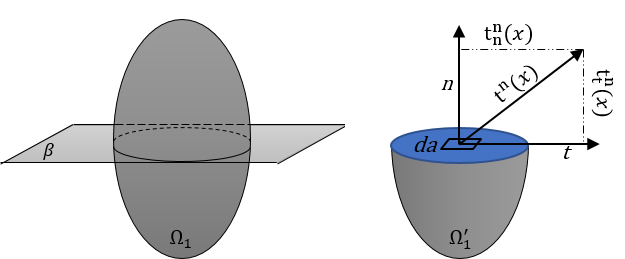
\includegraphics[width=0.7\textwidth,keepaspectratio]{figures/internalcontactForceDefinition.png} 
\caption[]{True stress vector $t^n(x)$ at point $x$ on the fictitious surface created  by the cutting plane $\beta$ of normal  $\overrightarrow n$ passing through the point $x$. }
\label{internalcontactForceDefinition}
\end{center}
\end{figure}

The stress on the boundary $\partial \Omega_1$ of the region occupied by the body is applied by external forces through physical contacts along the boundary. When formulating and solving a boundary-value problem, this stress defines the boundary conditions.


\subsubsection*{Cauchy's lemma}

Cauchy's lemma states that traction vectors acting on opposite sides of a surface are equal and opposite.
\begin{equation}
t^{-n}(x) = -t^n(x)
\label{chauchyLemma}
\end{equation}
\subsubsection*{Cauchy's Law}
Cauchy’s law states that it exists a Cauchy stress tensor $\sigma$ which maps linearly the normal to a surface to the stress vector acting on that surface, according to the next relation
\begin{equation}
t^n = \sigma \cdot n \ \ \ where \  \ t^n_i = \sigma_{i,j} n_j
\end{equation}

When large deformations are considered, the reference and current configurations of the body are significantly different and a clear distinction has to be made between them. The traction vector $t^n$ is defined in Eulerian coordinates (body current configuration) and is also called the \textbf{true stress}. Accordingly, the Cauchy stress tensor $\sigma$ is called the true stress tensor.

The definition of any measure with respect to the deformed configuration is less practical as it is usually unknown a priori. For the simplification of mathematical formulation, a new pseudostress is defined in the Lagrangian coordinate space named the \textbf{engineering stress}. The engineering stress has no physical meaning and has to be converted into true stress for any interpretation.


\begin{figure}
\begin{center}

\includegraphics[width=0.7\textwidth,keepaspectratio]{figures/stressnotion.png} 
\caption[]{Deformation of area $dA$  into area $da$. The force $df$ acting on deformed area $da$ and the pseudoforce $d\tilde{f}$ acting on undeformed area $dA$}
\label{stressnotion}
\end{center}
\end{figure} 


Below, two pseudostress vectors are defined (Figure  \ref{stressnotion}):
\begin{itemize}
\item $T^N$ defined as the contact force $df$ per unit area $dA$ in reference configuration.
\item $\tilde{T}^N$ defined as the contact pseudoforce $d\tilde{f}$ per unit area $dA$ in reference configuration.  
\end{itemize}


Accordingly, two pseudostress tensors are defined based on pseudostress vectors:
\begin{itemize}
\item $T^N = P \cdot N$, $P$ is called \textbf{first Piola-Kirschoff stress tensor},
\item  $\tilde{T}^N = S \cdot N $, $S$ is called \textbf{second Piola-Kirschoff stress tensor}. 
\end{itemize} 
where $N$ is the normal vector of unit area $dA$ in the reference configuration.

The three stress tensors are linked by the next relation 
\begin{equation}
\sigma = J^{-1}F \cdot P = J^{-1} F \cdot S \cdot F^T
\label{PK12}
\end{equation}


\subsection{Conservation equations}\label{subsection:conservationequations}
Three conservation laws must be satisfied by physical system subject to any applied boundary conditions: \textbf{conservation of mass, conservation of linear momentum} and \textbf{conservation of angular momentum}. The resulting equations describe partially the mechanical behavior of a continuous body.

\subsubsection*{ Conservation of mass}
The mass $m$ of a body with the density $\rho$, that infills the space region $\Omega_1$ is given by :
\begin{equation}
m(\Omega) = \int_{\Omega} \rho(X)dV
\end{equation}
The mass conservation law requires that the body mass remains constant throughout all possible body configurations. In a Lagrangian formulation, this results in a relation between the body density in the reference configuration $\rho_1$ and the body density in the current configuration $\rho$.

\begin{equation}
\int_{\Omega_1} \rho_1 dv = \int_{\Omega_0} \rho_0 dV = const. 
\end{equation}


Using the relation \ref{JacobianRelation} one can deduce that:
\begin{equation}
\int_{\Omega_0} \left( \rho_1 J - \rho_0\right)dV = 0 \  \ and \  \ \rho_1 J = \rho_0
\end{equation}
\subsubsection*{Conservation of the linear momentum}
Let assume that the body $\mathcal{B}$ is defined on a arbitrary region $\Omega_0$ with a boundary $\Gamma_0$, and is subject to a body-force $\rho_0  b$ and the surface traction $T^N$. And let $X$ be the particle location in the undeformed solid.
 The total force acting on the body $\mathcal{B}$ is then defined as:
\begin{equation}
f = \int_{\Omega_1}\rho_0 b(X)dV + \int_{\Gamma_0} T^N(X)dA
\end{equation}
 
The conservation of the linear momentum requires the total force acting on the body to be equal to the time rate change of the linear momentum. In a static problem, the time rate change of the linear momentum is neglected and thus an equilibrium equation is obtained.
\begin{equation}
\rho_0 b+\nabla_0 \cdot P  = 0
\end{equation}
Where the $P$ is the first Piola-Kircchoff stress tensor.	
The equilibrium equation can be formulated in terms of the second Piola-Kircchoff stress tensor by using relations \ref{PK12} .
\subsubsection*{Conservation of angular momentum}
The conservation of the angular momentum requires that the resultant momentum on any part of the body about a fixed point $\mathcal{O}$ equals the rate of increasing its angular momentum (about $\mathcal{O}$). For a static problem, the integral form of the conservation of the angular momentum is defined as:
\begin{equation}
\label{angularMomentum}
\int_{\Omega_0} X \times \rho_0 b(X)dV + \int_{\partial \Omega_0} X \times  T^N(X)dA = 0
\end{equation}

The relation \ref{angularMomentum} requires that the second Piola-Kircchoff stress tensor is a symmetric tensor:
\begin{equation}
S = S^T
\end{equation}
In summary, the conservation equations are fulfilled if and only if the following local conditions are fulfilled at each point in the body:
\begin{equation}
\rho_1 J = \rho_0, \ \ \nabla_0 \cdot S \cdot F^T + \rho_0 b =0, \ \ S=S^T 
\end{equation}
with the traction on the surface related to the stress through $\tilde{T^n} = S \cdot N$.
 For the simplification of mathematical calculus, the constitutive equations are formulated in terms of the second Piola-Kircchof stress tensor using the relations \ref{PK12}.

\subsection{Constitutive models}\label{subsection:constitutivemodels}
   The constitutive models, called also material models, define the relation between stress and strain of a physical system under the action of external stimuli. It is almost impossible to define a universal material behavior capable to model the material response to all possible conditions. Thus, for a given material, several constitutive models can be defined depending on the studied characteristics. \\
	Biological materials are classified into:
	\begin{itemize}
\item \textit{ Isotropic or anisotropic materials:} in a isotropic (anisotropic) material the values of a property are constant (vary) with respect to the direction.

\item\textit{ Compressible or incompressible materials:} in a compressible (incompressible) material the volume changes (remains constant) during the deformation and the density remains constant. For an incompressible material the Jacobian determinant of the deformation tensor $J$ is equal to 1. 

\item \textit{Homogeneous or heterogeneous materials:} in a homogeneous (heterogeneous) material the values of a property are constant (vary) with respect to the position within the body.
	\end{itemize}

Biological soft tissues are modeled using elastic materials model. The elasticity is the property of a solid material to return to its original size and shape when the influence of an external force is removed. In this case the strains are said to be reversible. 
	 
Considering small deformations, the stress-strain law of a linear material is given by the \textbf{Hook's law}
\begin{equation}
sigma = \lambda \epsilon
\end{equation},where  the coefficient of proportionality $\lambda$ \nomenclature{$\lambda$}{Young's modulus} is named \textbf{Young's modulus}. 

 Elastic materials may be defined also with a non-linear stress-strain relationship. In such cases the elastic modulus ($\lambda $) is defined in function of strain $\epsilon$ 
 \begin{equation}
 \lambda = \frac{\partial \sigma}{\partial \epsilon} = f(\epsilon).
 \end{equation}

For example, for an elastic exponential material \citep{azar_methods_2002} the elastic modulus is computed using the function 
\begin{equation}
f(\epsilon) = b e^{m \epsilon},
\end{equation} 
where b and m are material parameters.
 
For large deformations the stress-strain relationship is deduced from a potential function. A \textbf{hyperelastic} material is an elastic material for which the work is independent of the deformation path. The material reversibility and path-independent behavior implies the absence of energy dissipation during the deformation. Thus, it exists a \textbf{potential} function $W(E)$ such that
\begin{equation}
 S = \frac{\partial W(E)}{\partial E}= 2\frac{\partial \psi (C)}{\partial C}.
\end{equation}

Moreover, if the material is isotropic, the stored strain energy $W$ of a hyperelastic material can by written as a function of principal invariants ($I_1, I_2, I_3$) of the Green deformation tensor $C$ previously defined in equation \ref{principal_invariants}.

We introduce below the most used potential functions for the characterization of biological soft tissues.
 
For the simplification of potential expressions, we define the first and the second deviatoric strain (strain related to the deformation at constant volume) invariants:

\begin{center}
\begin{equation}
\overline{I}_1=\frac{I_1}{I_3^{2/3}} ; \overline{I}_2=\frac{I_2}{I_3^{4/3}}
\end{equation}
\end{center}

We also define the \textbf{Bulk modulus} K \nomenclature{K}{Bulk modulus} as measure of a material's resistance to compression, the \textbf{shear modulus} $\mu$\nomenclature{$\mu$}{Shear modulus} as the ratio of shear stress to the shear strain, and the \textbf{Poisson ratio} \nomenclature{$\nu$}{Poisson ratio} as the ratio between longitudinal strain to the transverse strain describing the body shape change. For small deformations the Bulk modulus and the shear modulus are linked to the Young's modulus and the Poisson ratio by the following relations:
 \begin{equation} 
  K = \frac{\lambda}{3(1-2\nu)} \ \ and \ \ \mu = \frac{\lambda}{2(1+\nu)}
\end{equation}
  
\subsubsection*{Neo-Hookean potential function}
The Neo-Hookean \citep{treloar_elasticity_1943} law is an extension of the Hook's law to large deformations. The potential function is based only on the first invariant and is given by 
\begin{equation}
\label{eq:Neo-Hookmodel}
W =\frac{\mu}{2} (\overline{I}_1-3) + \frac{K}{2}(J-1)^2,
\end{equation}
where $\mu$ and $K$ are the initial shear modulus and the initial Bulk modulus respectively. 
\subsubsection*{Mooney-Rivlin potential function}
The potential function of a Mooney-Rivlin \citep{rivlin_large_1951} material can be defined as:
\begin{equation}
\label{eq:mooneyRivlingmodel}
W=\frac{\mu_1}{2}(\overline{I}_1-3)+\frac{\mu_2}{2}(\overline{I}_2-3)+\frac{K}{2}(J-2)^2,
\end{equation}
where the constants $\mu_1$ and $\mu_2$ describing the material properties are linked to the initial shear modulus $\mu = (\mu_1+\mu_2)$, and the constant $K$ is the initial Bulk modulus. 

\subsubsection*{Gent potential function}
The potential function of a Gent \citep{gent_forms_1958} material model is defined as:
\begin{equation}
\label{gentmodel}
W=-\frac{\mu J_m}{2}ln\left(1-\frac{\overline{I}_1-3}{J_m}\right)+\frac{K}{2}\left(\frac{J^2-1}{2}-lnJ\right),
\end{equation}
 where the constants $\mu$ and $K$ constants are the initial shear modulus and the initial Bulk modulus respectively. And $J_m$ is a parameter limiting the value of $(\overline{I}_1-3).$
\subsubsection*{Ogden model}
The Ogden \citep{ogden_large_1972} material model is based on the three principal stretches ($\lambda_1,\lambda_2,\lambda_3$) and $2N$ material constants, where $N$ is the number of polynomials that constitute the potential function:
\begin{equation}
\label{eq:ogdenmodel}
W= \sum^N_{i = 1} \frac{\mu_i}{\alpha_i}(\lambda_1^{\alpha_i}+\lambda_2^{\alpha_i}+\lambda_3^{\alpha_i}-3) + \sum_{k=1}^N \frac{K}{2}(J-1)^{2k},
\end{equation}
where $\mu_i$ and $\alpha_i$ are material constants, and $K$ is the Bulk modulus.

\subsubsection*{Yeoh model}
The potential function of Yeoh \citep{yeoh_characterization_1990} model is based on the first invariant:
\begin{equation}
\label{eq:yeohmodel}
W = \sum_{i=1}^N \mu_i(\overline{I}_1 - 3)^i + \sum_{k=1}^N \frac{K}{2}(J-1)^{2k},
\end{equation}
where the $\mu_i$ are material constants and $K$ is the Bulk modulus.

\subsubsection*{Governing equations of Lagrangian formulation} 
We consider a body $\mathcal{B}$ which occupies in the reference configuration the domain $\Omega_0$ with a boundary $\Gamma_0$. The governing equations for the mechanical behavior of a continuous body are:
\begin{enumerate}
\item Conservation of mass $\rho_1 J = \rho_0$
\item Conservation of linear momentum $\nabla \cdot P + \rho b = 0$
\item Conservation of angular momentum $F \cdot P = P^T \cdot F^T$
\item Constitutive equations
\item Measure of strain $E = \frac{1}{2} (C-I)$
\item Boundary conditions: $e_i \cdot N \cdot P = e_i \cdot \overline{t}$ on $\Gamma_0^{t_i}$
\item Internal continuity condition: $\llbracket e_i \cdot N \cdot P \rrbracket = 0$ on $\Gamma_0^{int}$
\end{enumerate} 

Where we note $\Gamma_0^{t_i}$ the set of prescribed tractions  $\overline{t}$ on the body boundary $\Gamma_0$ ; and $\Gamma_0^{int}$ is the union of all surfaces where the stresses are discontinuous in the body (material interfaces).

The momentum equation together with the traction boundary conditions and the interior traction continuity condition are called the generalized momentum balance (GMB) \nomenclature{GMB}{Generalized Momentum Balance}.
\section{Finite Element Discretization}

\label{section:lagrangianmesh}
In continuous mechanics the body deformation is expressed in terms of partial differential equations (PDE \nomenclature{PDE}{Partial Differential Equations}). For the majority of problems, the PDE cannot be solved analytically, therefore approximation methods are developed. To this end, the finite element (FE) method has become the standard numerical calculation to compute such approximations. The computational domain, the unknown solution, and its partial derivatives are discretized, so as to obtain a set of algebraic equations for the function values at a finite number of discrete locations. The unknowns of the discrete problem are
associated with a computational mesh which represents a subdivision of the domain $\Omega_0$ into many small control volumes $\Omega_k$

\subsection{Eulerian and Lagrangian mesh description}

The mesh description depends on the chosen independent variables (Eulerian or Lagrangian formulation). An Eulerian mesh formulation is usually used to solve problems linked to fluid like materials, and a Lagrangian mesh for solid like materials. In an Eulerian mesh, the Eulerian coordinates of nodes are fixed (coincident with spatial points) and the material points change in time (see Figure \ref{lagrangian_mesh}.b). In this case the mesh has to be large enough to contain the body in its current configuration. Throughout the deformation, the material points will belong to different elements. On the contrary, in a Lagrangian mesh, the Lagrangian coordinates of nodes are time invariant, nodal trajectory corresponds with material points trajectory and no material passes between elements (see Figure \ref{lagrangian_mesh}.a). 

\begin{figure}[!h]
\centering
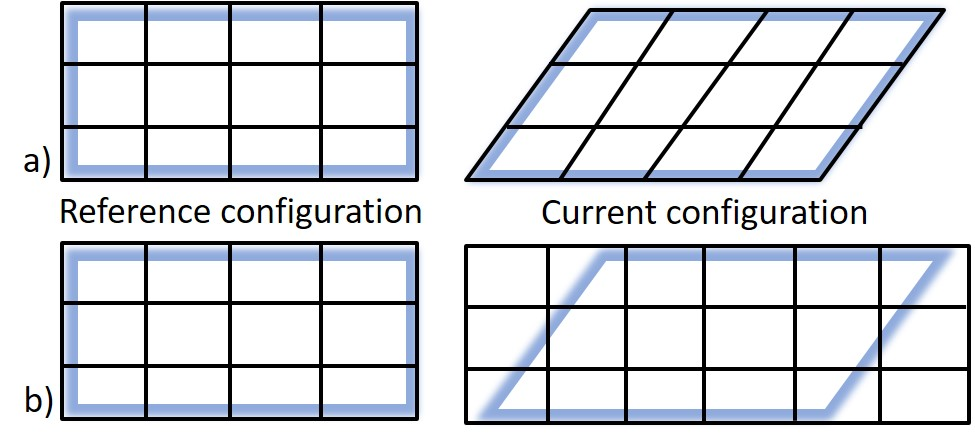
\includegraphics[width=0.8\textwidth,keepaspectratio]{figures/lagrangian_mesh.jpg} 
\caption{a) Lagrangian mesh formulation. b) Euler mesh formulation}
\label{lagrangian_mesh}
\end{figure}
 

In a Lagrangian mesh, the boundary and interface nodes remain coincident with body boundaries and material interfaces throughout the entire deformation. Thus, the boundary conditions are defined directly on the respective nodes. On the other hand, in an Eulerian mesh, the boundary and interface conditions have to be defined on points which are not nodes. This implies important complications in multi-dimensional problems.  

An important drawback of a Lagrangian mesh affects mainly the large deformation domain. As the nodes are coincident with the material points, the elements deform with materials. Therefore, the magnitude of deformation is limited because of the element distortion. The limited distortion that most elements can sustain without performance degradation or failure is an important factor in nonlinear analysis with Lagrangian formulation. 
 

\subsection{Lagrangian mesh}\label{subsection:lagrangianmesh}

The general approach of the FE method in Lagrangian formulation is illustrated in Figure \ref{fe_method}. First, the momentum equations with given boundary conditions are multiplied by a set of appropriate test functions. The test functions have to satisfy all displacement boundary conditions and to be smooth enough so that all derivatives in momentum equations are well defined. Then, performing an integration by parts, the weak formulation of GMB is obtained, also called the principle of virtual work \citep{belytschko_nonlinear_2013}. 

\begin{figure}[!h]
\centering
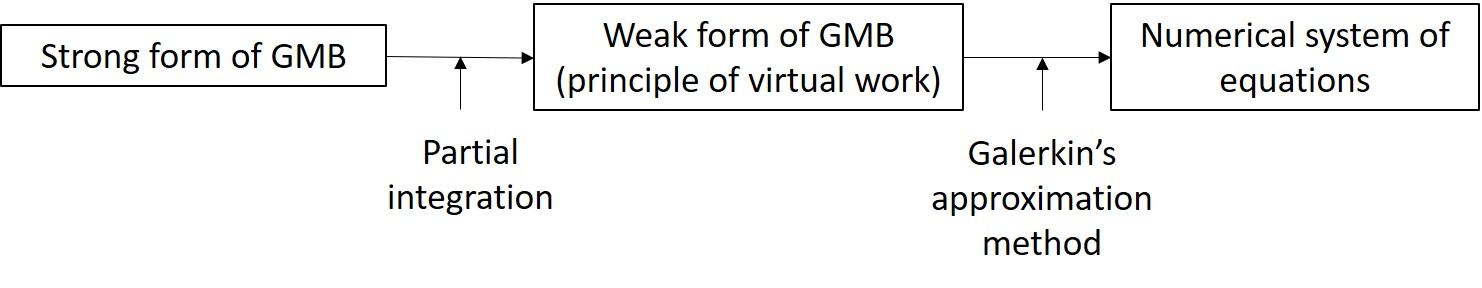
\includegraphics[width=0.8\textwidth,keepaspectratio]{figures/fe_method.jpg}
\caption{From strong formulation of the generalized momentum balance (GMB) to numerical equations.}
\label{fe_method}
\end{figure}




 The momentum equations and the traction boundary conditions, usually called the strong form, cannot be directly discretized by an FE method. The strong formulation of the GMB equations imposes the $C_1$ continuity conditions on the field variables. Therefore, the solution of this problem does not always exist. This is true especially in the case of complex domains with different material interfaces. In order to overcome these difficulties, weak formulations are preferred. The weak formulation of the GMB reduces the continuity requirements thereby allowing the use of easy-to-construct and implement polynomials. Due to reduced requirements in function smoothness, the weak forms never give an exact solution, but one can obtain a relatively accurate solution with the discretization refinement.



From the weak form of the GMB equations, the numerical system of equations is formulated by using finite element interpolants for the mechanical displacement and the test functions.   The whole domain is discretized into a number of smaller areas or volumes which are called \textbf{finite element} (or elements) and their assembly is called a\textbf{ mesh}. Finite elements can be of various shapes (as shown in Figure \ref{discretization}.b),  quadrilateral or triangular in two dimensions, and tetrahedral or hexahedron in three-dimensions.


\begin{figure}[!h]
\centering
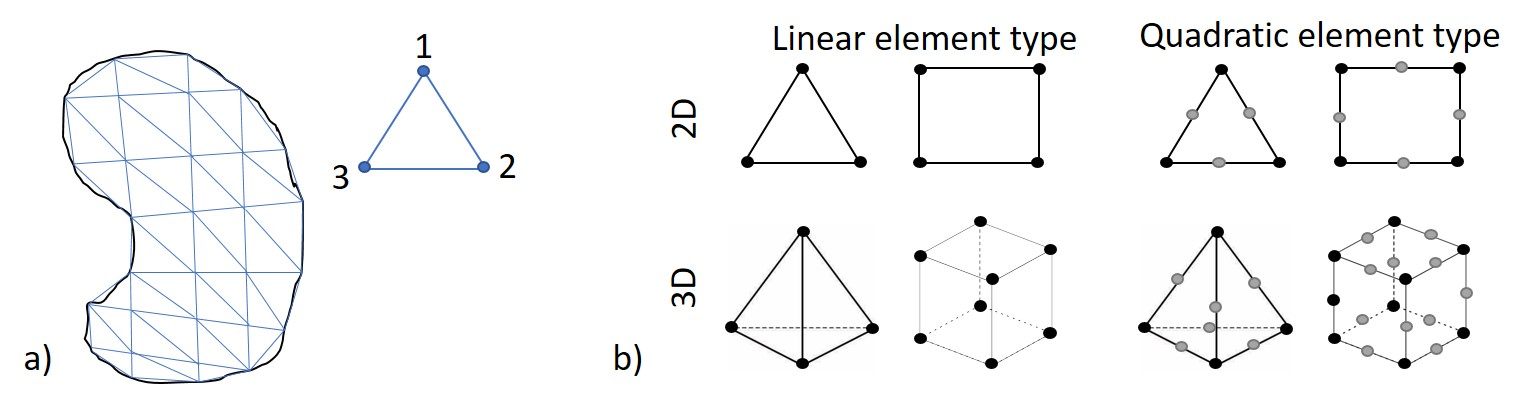
\includegraphics[width=1\textwidth,keepaspectratio]{figures/discretization.jpg} 
\caption{a) Discretization of  a 2D domain with triangular finite element: Lagrangian mesh. b) Different types of finite elements}
\label{discretization}
\end{figure}

 The mechanical displacement is approximated at the discretization points called finite element \textbf{nodes}. The nodes are at the vertices of the finite elements for a linear type, and at the vertices and mid-side of the finite element edges for a quadratic type (Figure \ref{discretization}.b). The displacement of each point within an element is interpolated from the values of the displacements of the nodes of the this element. In this way, the problem of finding the displacement of every point within the body is replaced by the problem of finding the displacements of a finite number of nodes.
 
 As in a Lagrangian mesh the nodes are following the motions, for large deformations the finite elements can be highly distorted. Therefore, the element shape quality is generally checked all along the deformation process. Several shape parameters for each element type have been proposed, such as: aspect ratio, maximum corner angle, Jacobian ratio, skewness, parallel deviation, warping factor. The acceptable limit values of these shape factors are proper to the element types.
In the following, only the shape parameters of the linear triangular elements are presented \citep{ansys_theory_2017}.  
 \subsubsection*{Triangle aspect ratio }
 The element's shape aspect ratio is computed using only the vertices, corner nodes, of the element (Figure \ref{fig:aspectratio}). First, two lines are created: one through a node ($K$) and the midpoint of the opposite edge ($ K'$), the second through the midpoint of the others two edges ($J'$ and $ I'$). Then two rectangles are created, with each rectangle having a pair of edges parallel to one of the previously defined lines. The rectangle edges have to pass through the nodes and the triangle's edge midpoints. This construction is repeated for each triangle's node resulting in 6 rectangles. The aspect ratio of a rectangle is defined as the ratio between the longer and shorter sides. Thus, the triangle's aspect ratio is defined as the maximal aspect ratio over the 6 rectangles divided by squared root of 3. 
 
 The best possible aspect ratio is 1 and is represented by an equilateral triangle. An element with an aspect ratio larger than 20 is considered as a bad aspect element, because large aspect ratio may degrade solution performance.
 
 \begin{figure}[!h]
\centering
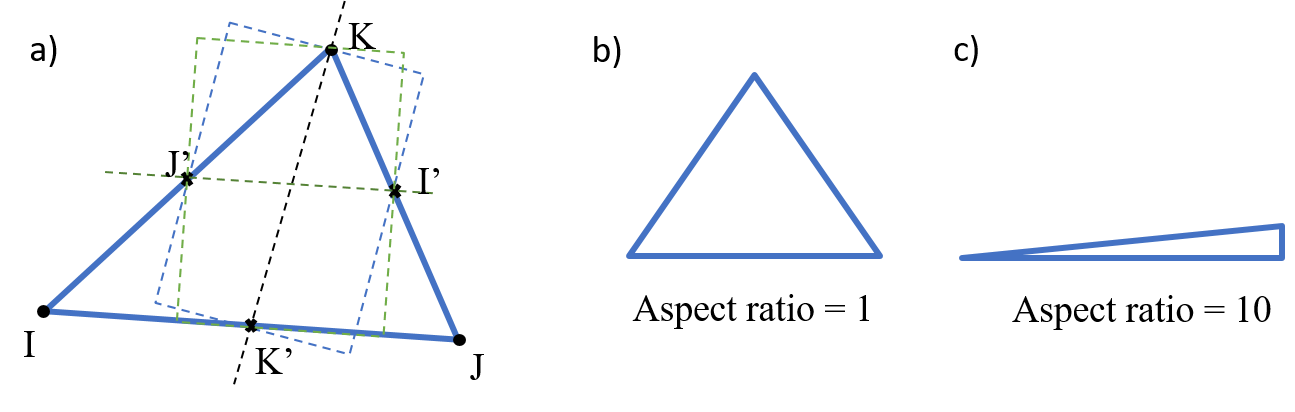
\includegraphics[width=0.9\textwidth,keepaspectratio]{figures/aspectRatio.png} 
\caption{Computation of the aspect ratio for a triangle}
\label{fig:aspectratio}
\end{figure}  

\subsubsection*{Triangle maximum corner angle}
The maximum corner angle is computed using nodes position in 3D space. The best possible maximum corner angle is 60\textdegree. An element having a maximal corner angle larger than 165\textdegree is considered as a bad shape element, because large corner angles may degrade the solution performance. Figure \ref{fig:cornerangle} shows a triangle with a good ( 60\textdegree) and bad ( 165\textdegree) quality. 

 \begin{figure}[!h]
\centering
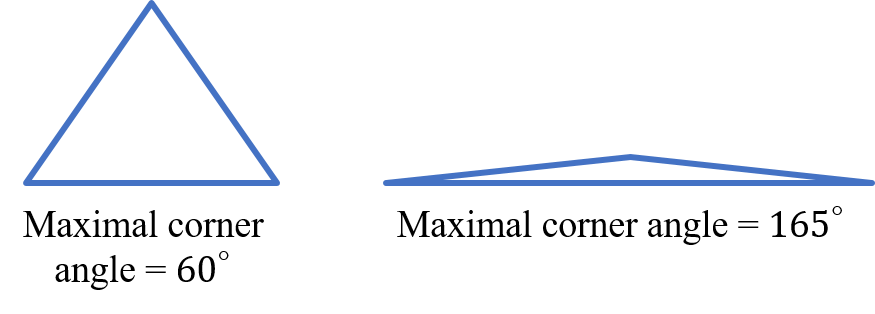
\includegraphics[width=0.6\textwidth,keepaspectratio]{figures/maximalcornerangle.png} 
\caption{Example of triangles with different maximal corner angles.}
\label{fig:cornerangle}
\end{figure} 

The aspect ratio and the maximal corner deviation of a tetrahedra is computed using the definition of the same measure on a triangle. The element shape parameter is assigned as the worst value over the triangles defined by the tetrahedra's faces and cross-sections.  

\subsubsection*{Skewness }
The skewness of a triangular element is computed using the equivalent volume deviation method. It is defined as the difference between the optimal and the real cell size over the optimal cell size. The optimal size is the size of an equilateral cell with the same circum radius. According to its definition, the value of 0 indicates an ideal cell, from 0 to 0.75 the cell is considered to have a good quality, from 0.75 to 1 the cell is considered to have a bad quality and a value of 1 indicates a completely degenerated cell (Figure \ref{fig:skewness}).   

 \begin{figure}[!h]
\centering
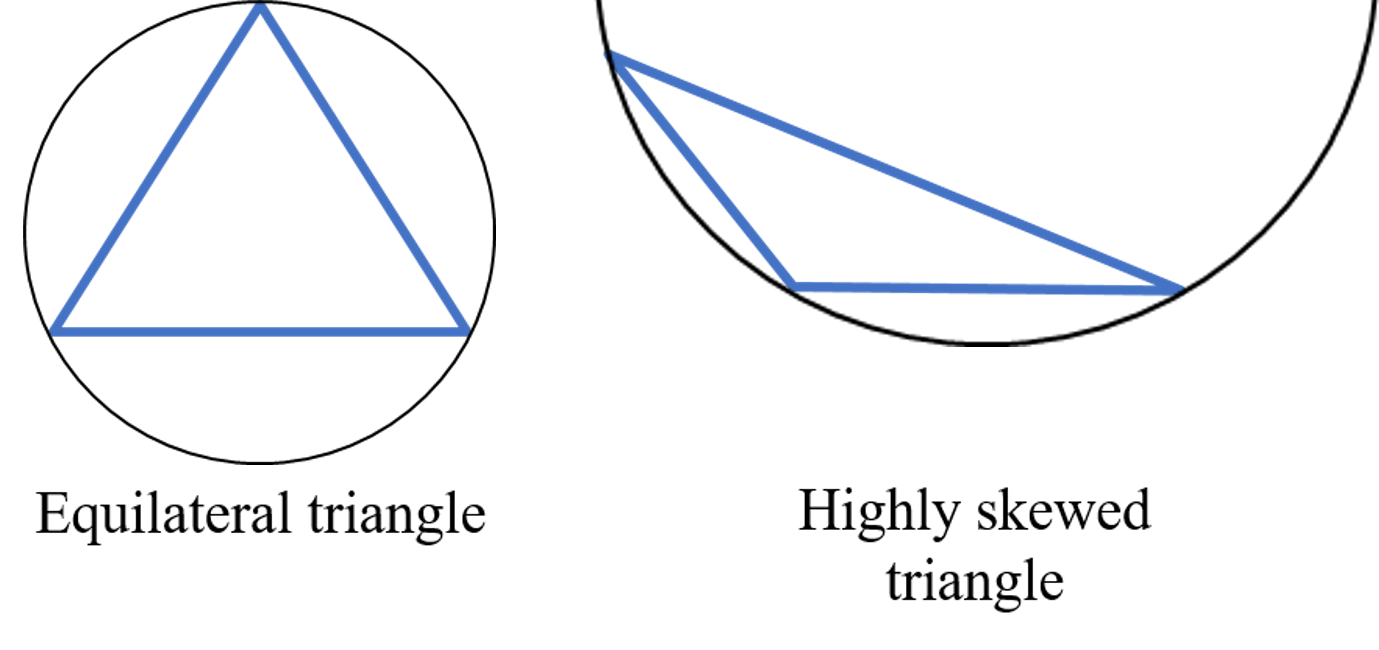
\includegraphics[width=0.6\textwidth,keepaspectratio]{figures/skewness.png} 
\caption{Example of triangles with different skewness with the corresponding circum radius.}
\label{fig:skewness}
\end{figure}
 
\section{Contact mechanics}\label{section:contactmechanics}

In order to transfer the loads between elements, the nodes have to be connected together. If two bodies are separated with no common nodes, no interaction will occur during the deformation and the bodies will pass through each other. Here, an asymmetric surface-to-surface contact method is used to solve the multi-body interaction problems.

Let's consider two different bodies $\mathcal{A}$ and $\mathcal{B}$ and their occupied domains $\Omega_A$ and $\Omega_B$ with boundaries $\Gamma_A$ and $\Gamma_B$ respectively (see Figure \ref{contact_bodies}). Also, we note $\Omega$ the domain of intersection of two bodies. The contact interface is the intersection of the surfaces of the two bodies:
\begin{equation}
\Gamma = \Gamma_A \cap \Gamma_B.
\end{equation}

The intersection consists of two surfaces, usually distinguished as \textbf{target} and \textbf{contact} surfaces. For an asymmetric contact each surface has a single designation and the choice of the surface types is made following these next guidelines (the target surface properties are enumerated in their priority order):
\begin{itemize}
\item If the body $\mathcal{A}$ is stiffer than the body $\mathcal{B}$, the surface $\Gamma_A$ defines the target and $\Gamma_B$ the contact surface.
\item If $\Gamma_A$ is a concave surface getting in contact with the convex surface $\Gamma_B$, the surface $\Gamma_A$ defines the target and $\Gamma_B$ the contact surface.
\item If $\Gamma_A$ is larger than $\Gamma_B$, the surface $\Gamma_A$ denotes the target and the surface $\Gamma_B$ the contact surface.
\end{itemize} 
For the following, we identify $\Gamma_A$ as the target surface and $\Gamma_B$ as the contact surface (Figure \ref{contact_bodies}). 

 Sometimes, the asymmetric contact does not provide satisfactory results and a symmetric contact is needed. When defining a symmetric contact, each surface coming in contact is designated to be both contact and target surface types. Therefore, two sets of contact pairs are defined. The symmetric contact may be used when the distinction between the contact and the target surfaces is not clear or to reduce the contact penetration. However, it usually results in a more time-consuming solution.



\subsection{Contact inteface equations}%\label{governingequations}
 In the case of multi-body interaction, besides the standard mechanical governing equations, two additional contact conditions have to be fulfilled: the two bodies cannot interpenetrate, and the traction must satisfy momentum conservation on the contact interfaces.
   

\begin{figure}[h]
\centering
\centerline{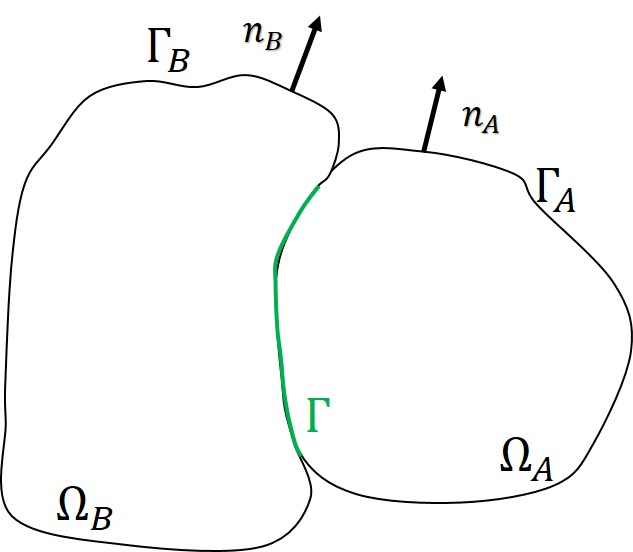
\includegraphics[width=0.4\textwidth,keepaspectratio]{figures/contact_bodies.jpg} }
\caption{Multi-body contact problem.}
\label{contact_bodies}
\end{figure}

   
  \subsubsection*{Traction conditions}
  Traction conditions must follow the balance of momentum across the contact interface:
  \begin{equation}
  t_A + t_B=0
\end{equation}
On the contact boundary surface $\Gamma$, the traction vector is decomposed into its normal and tangential components:

$$t_A^n = t_A \cdot n_A,  \ \ \ t_B^n = t_B \cdot n_B$$
$$t_A^t = t_A - t_A^n n_A, \ \ \ t_B^t = t_B - t_B^n n_B$$

Therefore the momentum balance requires:
\begin{equation} 
t_A^n + t_B^n = 0, \ \ \ t_A^t + t_B^t = 0
\end{equation} 

 \subsubsection*{Inter-penetrability condition}
The bodies implied in a multi-body problem must fulfill the inter-penetrability condition:
\begin{equation}
\Omega_A \cap \Omega_B = 0
\end{equation}
Decomposing the displacement $u$ into its normal and tangential components, $u^n$ and $u^t$ respectively, the inter-penetrability condition can be written as:
\begin{equation}
t^n \leq 0, \ \ u^n-g n_A \leq 0, \ \ t^n(u^n-g n_A) = 0
\end{equation}
 Where $g$ is the gap between the two bodies and $n_A$ is the normal to the target surface.

\subsection{Surface interaction models}%

\label{subsection:surfaceinteractionmodels}
When two solid bodies are placed together under a nonzero normal force and act one over the other with a tangential force, a \textbf{friction force} ($f_{friction}$) tangential to the interface and opposite to the applied force is created. Depending on whether the applied force can overcome  or not the opposing friction force, the bodies may or may not move relative to each other. The body motion along the interface is called \textbf{sliding}. The \textbf{sliding force}, $f_{sliding}$ is the resulting tangential force which causes the sliding motion between the two bodies.
  
According to the allowed relative body motion in tangential or normal directions, five types of surface interaction models can be distinguished: bonded, rough, no-separation, frictional and frictionless. Table \ref{contactB} resumes each corresponding mechanical behavior. If the body motion is not allowed in normal or tangential directions, once the bodies get in contact, the respective components of traction are equals ($t_A=t_B$). This means that, for a pure \textbf{bonded} contact, the two bodies are considered as a unique solid body.    

\begin{table}[H]

\begin{center}
\begin{tabular}{||c|c|c||}
\hline
Name & body motion in normal direction & body motion in tangential direction \\
\hline\hline
Bonded & No & No\\
\hline
Rough & Yes & No, $f_{friction} \gg f_{sliding}$ \\
\hline
No-separation & No & Yes, $f_{friction} = 0$ \\
\hline
Frictionless & Yes & Yes, $f_{friction} = 0$ \\
\hline
Frictional & Yes & Yes, if $f_{sliding} > f_{friction}$\\
\hline
\end{tabular}
\caption{Surface interaction models and corresponding mechanical behaviors}
\label{contactB}
\end{center}
\end{table}

The \textit{frictional} contact behavior is defined using Coulomb friction law. For a continuous body, the Coulomb friction model is applied at each point of the contact interface.
Considering that bodies $\mathcal{A}$ and $\mathcal{B}$ are in contact within the surface $\Gamma$, then for all $x \in \Gamma$:
\begin{equation}
\label{stiking}
if \ \Vert t^t(x) \Vert < -\mu_f t^n(x),\ \ \Delta u^t=0 
\end{equation}
\begin{equation}
\label{sliding}
if \ \Vert t^t(x) \Vert = -\mu_f t^n(x),\ \ \Delta u^t=-k(x)t^t(x),\ \ k(x)>0
\end{equation}

Where $\mu_f$ is the material property named \textbf{friction coefficient},  $\Delta u^t$ is the slip incremental in the tangential direction and $k(x)$ is a variable computed from the momentum equation. The equation (\ref{stiking}) is known as the sticking condition: the tangential traction is lower than the critical value, thus no sliding occurs. Reciprocally, equation (\ref{sliding}) is called the sliding condition.

When a frictionless contact model is used, $\mu_f = 0$, the tangential tractions vanish completely: $t_A^t = t_B^t = 0$. On the contrary, when a rough contact is modeled, the friction coefficient $\mu_f$ is equal to infinity, so that the sticking condition is always fulfilled. 

In practice, several contact models can be combined to model a physical contact between two bodies.   

\subsection{Contact formulation algorithm: pure penalty model}%\label{subsection:purepenalty}

\subsubsection*{Pinball region}

Contact formulation presents two primary difficulties from a computational point of view. The first, is the unknown traction conditions for each considered frictional model. And second, the regions which will get in contact during the deformation process can not be predicted.

The region of contact depends on materials properties and imposed boundary conditions. Therefore, it is difficult to know a priori where the surfaces will be in contact. To formulate analytic equations, one has to know exactly the nodes involved in the contact process. Therefore, during body deformation, the program searches if the contact is \textit{opened} or \textit{closed}. The status is defined using a sliding pinball (Figure \ref{fig:pinball}). The pinball slides over the contact surface nodes and searches for the target surface. If the node to surface distance is smaller than the pinball radius, the contact is considered to be closed (Figure \ref{fig:pinball}, green nodes). Otherwise the contact is considered to be opened (Figure \ref{fig:pinball}, gray nodes).    

\begin{figure}[!h]
\centering
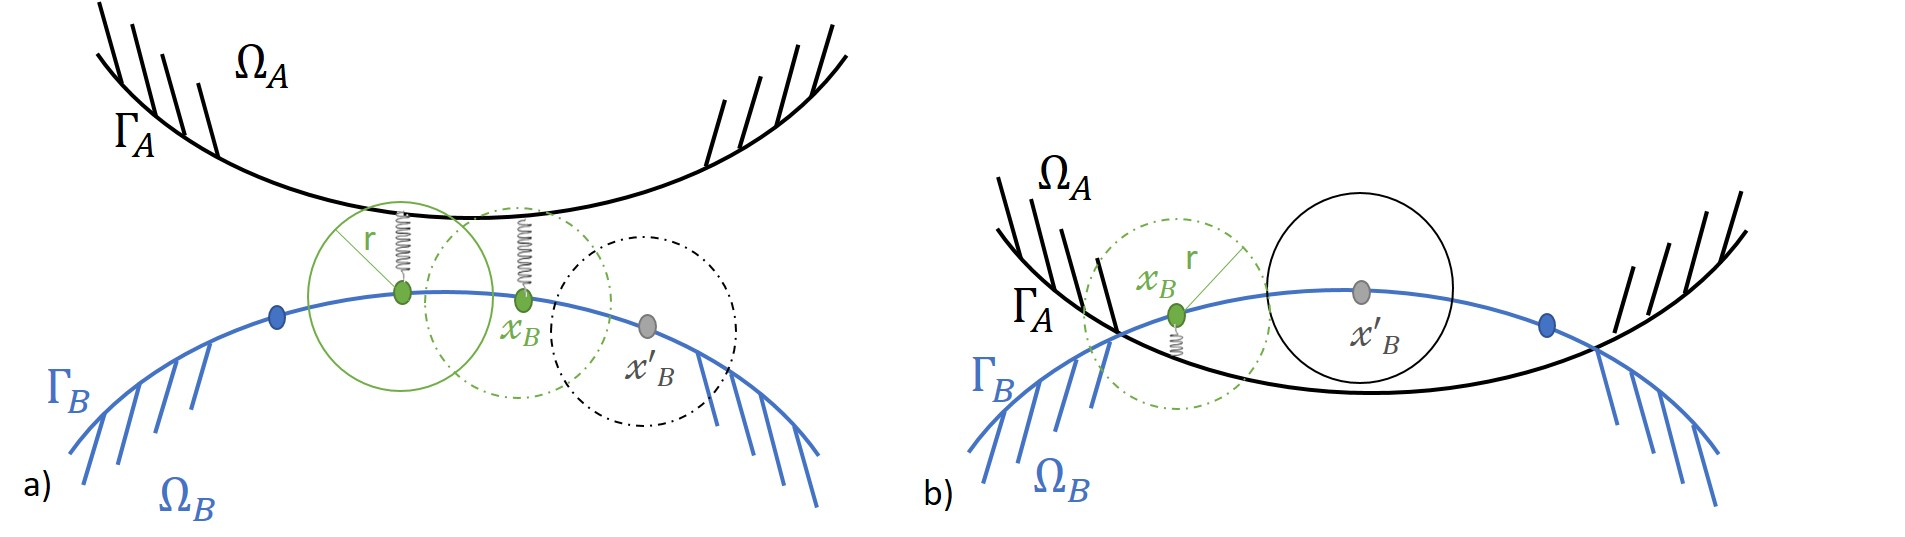
\includegraphics[width=1\textwidth,keepaspectratio]{figures/pinball.jpg} 
\caption{Contact status update using a pinball of radius r. Green nodes - updated nodes to closed contact status; gray nodes - updated nodes to open contact status; blue nodes - nodes which contact status need to be updated}
\label{fig:pinball}
\end{figure}

 
 \subsubsection*{Gap and penetration measures} 
  Let's consider a point $x_B$ belonging to the body surface $\Gamma_B$, and $x_A$ the intersection point of the surface normal $n_B$ with the surface $\Gamma_A$ (Figure \ref{gap_penetration}). The point to surface distance $d_1(x_B,\mathcal{A})$  is defined as:
\begin{equation}
\label{normalContactdistance}
d_1(x_B,\mathcal{A}) = \Vert x_B-x_A \Vert = \left[  \Sigma_{i={1,2,3}}\left( x_B^i - x_A^i \right)^2\right]^{\frac{1}{2}}
\end{equation}


\begin{figure}[!h]
\centering
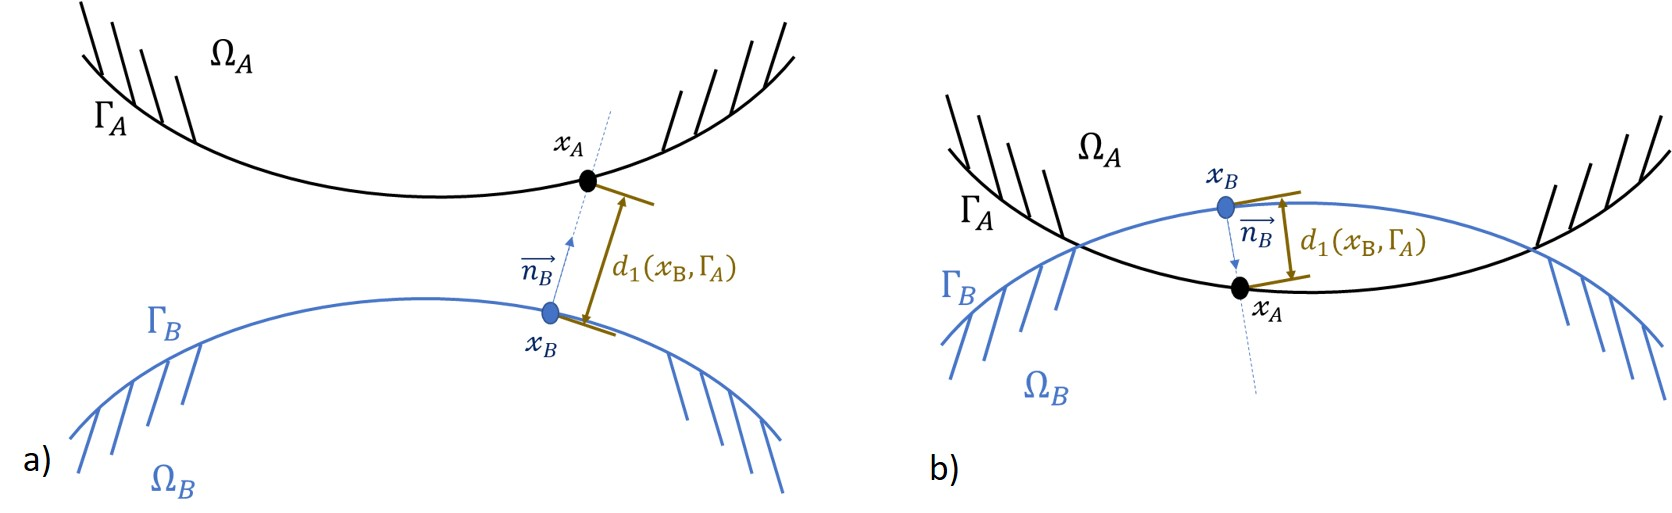
\includegraphics[width=1\textwidth,keepaspectratio]{figures/gap_penetration.jpg}
\caption{a) Body $\mathcal{A}$ and body $\mathcal{B}$ are close but not in contact. The $d_1(x_B,\mathcal{A})$ measure define the gap between the bodies at point $x_B$.  b) Body $\mathcal{B}$ have penetrated the body $\mathcal{A}$. The $d_1(x_B,\mathcal{A})$ measure gives the penetration at point $x_B$.}
\label{gap_penetration}
\end{figure}

If the intersection point $x_A$ is located inside the pinball area, the node to surface distance defines the amount of \textbf{gap} or \textbf{penetration} of the respective node (Figure \ref{gap_penetration}).
 
Computing the gap or the penetration at single points increases numerical instabilities.  Therefore, in this work, surface projection based contact method proposed by ANSYS was used. In Figure \ref{fig:projecte_surface} the computation method of each projected area over the contact surface is explained. Figure \ref{fig:projecte_surface}.a represents the contact surface elements and Figure \ref{fig:projecte_surface}.b represents the target surface elements.  If the two surfaces are overlapped, each unique area becomes a surface projected contact area (Figure \ref{fig:projecte_surface}.c). Therefore instead of calculating  the penetration or the gap at each element node, the method computes an average value for each overlapping area.


\begin{figure}[!h]
\centering
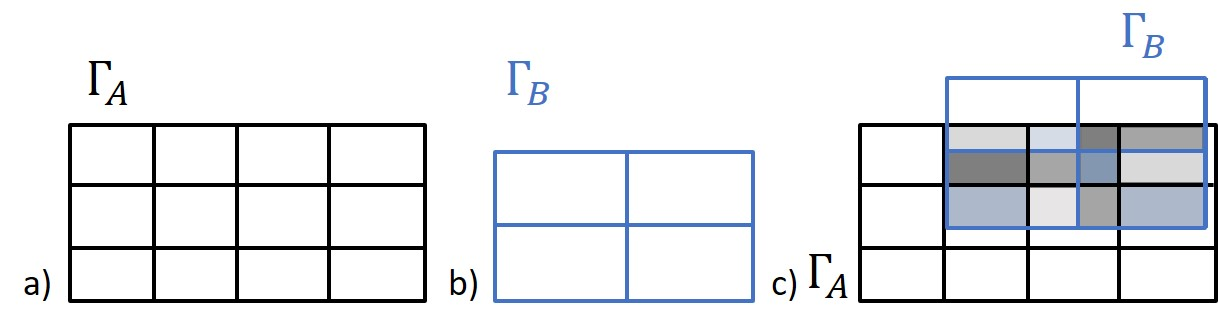
\includegraphics[width=1\textwidth,keepaspectratio]{figures/projecte_surface.jpg} 
\caption{The contact surface projection over the target surface: a) Target surface elements; b) contact surface elements; c) surface projected contact areas.}
\label{fig:projecte_surface}
\end{figure}

This approach provides a more accurate calculation of contact traction and stresses for the underlying elements, however it is computationally more expensive. The interested reader is referred to ANSYS contact technology guide \citep{ansys_contact_2017} for more details on the contact modeling.


\subsubsection*{Finite element mesh}
For the finite element computation, contact and target surfaces have to be discretized with 2D linear or quadratic elements (Figure \ref{discretization}) consistent with the underling 3D element mesh. The elements are named contact and target elements respectively.  They have no material properties apart the friction coefficient $\mu_f$. The stress-strain as well as the gap or penetration measures are computed for each mesh node of the discretized surface.

\subsubsection*{Pure Penalty method}
In this manuscript, one of the most popular mathematical expression of contact compatibility conditions is used, namely the penalty method. With such a method, additional contact properties are defined to manage contact behavior: a normal stiffness factor, opening stiffness factor, and a tangential stiffness factor. Such factors play an important role in the numerical computation but have no physical meaning.

The penalty method uses a spring like relationship to introduce a force for all nodes pairs (contact-target) that are defined to be in closed contact (Figure \ref{normalContactdistance}). The contact force is computed using the following expression:
\begin{equation}
f_c = k_c d
\end{equation}
where $d$ represents the penetration or gap amount and $k_c$ is the normal stiffness factor or the opening stiffness factor respectively. The tangential stiffness factor works in the same way enforcing the responding frictional force. Even if physical contacting bodies do not interpenetrate ($d = 0$), some finite amount of penetration, $d > 0$, is required mathematically to maintain equilibrium. 
 
 The magnitude of the stiffness contact factors is unknown beforehand which makes difficult a proper estimation of contact mechanics. The contact force at each node has to be large enough to push the contact surface back to the target surface and eliminate unwanted penetration or gap. At the same time, if the contact force is too large, it pushes the contact surface far away from the pinball region causing error and solution instabilities.

\section{Breast biomechanical model: an overview}

Biomechanical modeling of breast tissues has been widely investigated for various medical applications such as surgical procedure training, pre-operative planning, diagnosis and clinical biopsy, image guided surgery, image registration, and material parameter estimation (Table \ref{table:mechanical_models_table}). For the last 20 years, several research groups have presented their breast models based on finite element theory.  The complexity and relevance to breast anatomy of each model depend on the research purpose for which it was designed. 

Several groups have proposed biomechanical breast models to register uncompressed volumetric breast data sets to compressed ones \citep{han_development_2012,ruiter_model_based_2006,sturgeon_finite_element_2016} or to compressed  mammography projections \citep{kellner_simulation_2007}. Within this framework, the authors modeled the breast deformation from prone to compressed prone position assuming linear elastic materials, zero residual stress and Dirichlet boundary conditions.
However, compression-like breast deformation is too limited to characterize global breast mechanics.

 Applications such as image guided surgery or preoperative planning imply a wider range of deformations. Therefore biomechanical breast models capable of estimating gravity induced deformation between different body position were proposed, for example from supine to prone positions (named also multi-loading gravity simulations) \citep{gamage_modelling_2012,georgii_simulation_2016,eiben_surface_2016}. Considering the involved large deformations, these models need to be more accurate with respect to mechanical and anatomical breast properties. In this respect, a patient-specific model is needed considering more personalized boundary conditions, material models and a better representation of breast anatomy. 

 
As described in Section \ref{section:continuousmechanics}, to build such a mechanical breast model, one needs to provide the breast geometry in a \textbf{reference configuration}, the \textbf{constitutive models} of tissues composing the breast volume and the \textbf{boundary conditions}. A proper definition of all these variables has a significant impact on model accuracy.

\subsection{Breast reference configuration} 

A large number of existing patient specific models are using volumetric data from MR images \citep{carter_biomechanical_2009,kellner_simulation_2007, conley_realization_2015, eiben_symmetric_2016, martinez_finite_2017}  or CT images \citep{palomar_finite_2008, sturgeon_finite_element_2016} to design the breast geometry. During the acquisition of such images, the breast tissues are already under large deformations implying significant changes of breast geometries, for example if the patient is in a supine or in a prone position. Moreover, the deformed breast configurations include already the initial pre-stresses which are generally unknown and are extremely difficult to measure in clinical conditions. 
 

To model the breast tissues deformation under gravity loading, the reference state is chosen to be the breast geometry in a stress-free configuration, i.e. without being deformed by any force, including gravity. The breast stress-free geometry is practically impossible to measure; therefore, several estimation methods have been proposed. The four most used methods are described below.

 
 
  \subsubsection*{Inverse gravity}\label{subsubsection:inversegravity}
Palomar A.P. et al. \citep{palomar_finite_2008} and Sturgeon G.M. et al. \citep{ sturgeon_finite_element_2016} used the inverse gravity method to estimate the stress-free geometry from the prone position measured using MRI modality. In their works, the authors just reversed the gravity effects without considering the initial stresses already included in the breast prone configuration. However, it has been proved that the inverse gravity method gives a poor approximation of the breast reference state and can be used only with small deformations or highly constrained models \citep{eiben_breast_2014}.  

 \subsubsection*{Breast neutral buoyancy configuration}
 Assuming that breast density is equal to water density, Rajagopal V. et al. \citep{rajagopal_creating_2008} compute the breast stress-free configuration by imaging the breast immersed in water. Following the same physical assumptions, Kuhlmann M. et al. \citep{kuhlmann_mechanical_2013} proposed to estimate the stress-free configuration by applying a hydro-static distributed load on the breast surface collected in a prone configuration. Although the estimated geometries are relatively accurate, these methods are time-consuming and are difficult to transpose in a clinical framework. 

 \subsubsection*{Prediction-correction iterative algorithm}
 The prediction-correction iterative method was first proposed by Govindjee S. and Mihalic P.A. \citep{govindjee_computational_1998} and adapted later by Carter T. \citep{carter_biomechanical_2009} and Eiben B. et al. \citep{eiben_breast_2014}. The original method is based on the prediction-correction iterative scheme represented in Figure \ref{predictioncorectionalgo}. The first approximation of the breast reference configuration is estimated by applying the inverse gravity method on the prone breast configuration (see above).  Then, a numerical breast prone configuration is computed and compared to the corresponding measured one. The difference between the two prone geometries (the measured one and the simulated one) is used to update the reference breast configuration. The process is repeated until the convergence is achieved (i.e. when the difference is minimal). These methods were validated using the breast shape in the neutral buoyancy configuration.

\begin{figure}[!h]
\centering
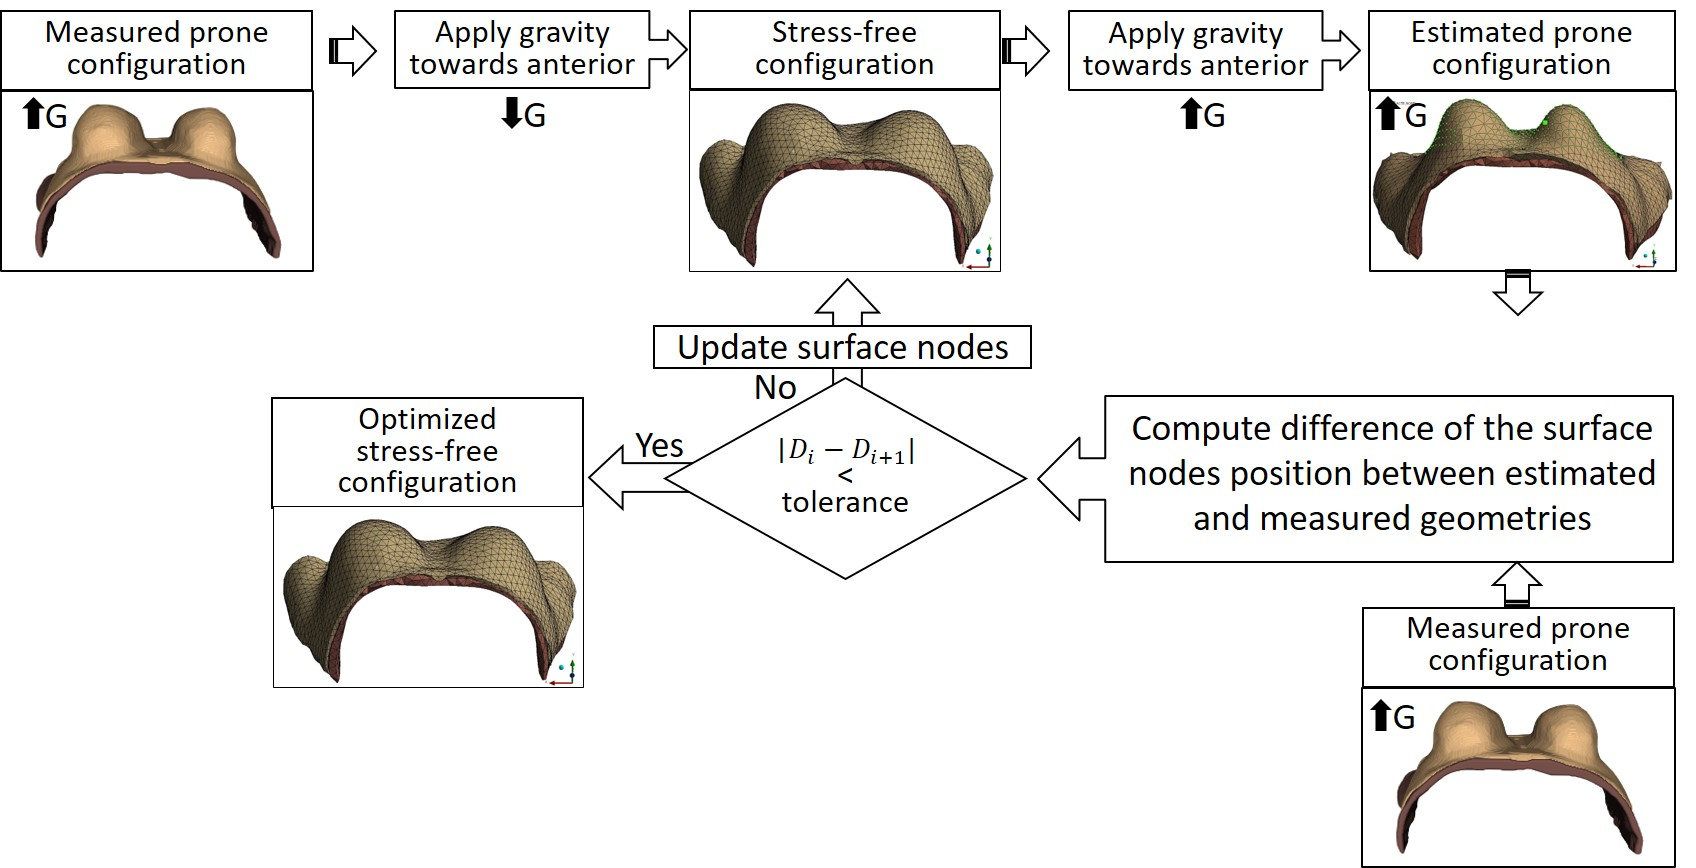
\includegraphics[width=1\textwidth,keepaspectratio]{figures/prediction-correction.jpg} 
\caption{Prediction-correction algorithm}\label{predictioncorectionalgo}
\end{figure}


 \subsubsection*{Inverse FE algorithm}
Pathmanathan P. et al. \citep{pathmanathan_predicting_2008} and later Vavourakis V. et al \citep{vavourakis_inverse_2016} proposed an analytic computation of the breast reference state by reparametrizing the equilibrium equation and by solving a finite element formulation of the inverse motion. The model provides good estimates of breast reference configurations but needs important numerical resources. Eiben B. and colleagues \citep{eiben_breast_2014} showed that the prediction-correction iterative algorithm and the inverse FE algorithm are similar in terms of resulting accuracy. 

\subsection{Constitutive models}

Global breast mechanics is governed by breast internal consistency and tissues' individual mechanical properties. The breast soft tissue is known to be incompressible, nonlinear, anisotropic, and viscous materials. However, even for small time scales loads the breast tissues viscosity can be neglected \citep{wellman_breast_1999}.  

Under large compressions, the breast volume can vary due to fluids (blood and lymph) flows. Thus, soft tissues are not considered as totally compressible materials, and are frequently modeled as quasi-incompressible with a value of the Poisson ratio $\nu$ ranging between $0.45$ and $0.5$. The influence of the Poisson ratio within linear constitutive models was studied by Tanner C. and colleagues \citep{tanner_factors_2006}; according to the authors, the best breast geometry estimates are obtained with high Poisson ratio ($\nu = {0.495-0.499}$). The breast tissues being predominately composed of water, the density is considered to be equal to $981\ kg/m^3$.  


For the last decades, several constitutive models were used to model the breast tissues response to an external force: exponential elastic \citep{azar_methods_2002}, Neo-Hookean hyper-elastic \citep{carter_biomechanical_2009,rajagopal_modeling_2010,sturgeon_finite_element_2016, eiben_breast_2016, han_nonlinear_2014, garcia_mapping_2017} and Mooney-Rivlin models \citep{samani_elastic_2007,tanner_factors_2006,carter_application_2012,martinez_finite_2017}. 
The most used models are analyzed in the following section.
 
\subsubsection*{Glandular and adipose tissues biomechanical properties }
 Multiple studies have shown that breast composition, and therefore its mechanical behavior, undergo substantial changes during woman lifetime (section \ref{subsection:adultbreasttexturechanges}). The first studies on mechanical proprieties estimation of breast tissues were done for diagnosis purposes. When the breast is developing benign or malign disorders, its mechanical properties differ from the ones of the normal breast tissues \citep{krouskop_elastic_1998}.  

Later, several research groups (Table \ref{table:materialproperties}) have studied the elastic modulus of adipose and glandular tissues. The breast tissue Young's modulus range between $0.1\ kPa$ and $271.8\ kPa$. Such huge variation may be explained by the differences in the experimental setups used to estimate tissues stiffness, but also by the participant's physical condition, age or period in the menstrual cycle. For example, Han L. et al. \citep{han_development_2012}, though using the same FE method, found significantly inter-individual variability, with the shear modulus ranging between $0.22$ and $43.64\ kPa$. Lorenzen J. and team \citep{lorenzen_menstrual-cycle_2003}, showed that during the menstrual cycle, due to the hormonal changes, the elastic properties of the glandular tissues can change by about $30\%$.

\begin{table}[!h]
\centering
\begin{tabular}{|p{0.25\linewidth}|p{0.13\linewidth}|p{0.1\linewidth}|p{0.17\linewidth}|p{0.17\linewidth}|}
 \hline
\multicolumn{5}{|c|}{\textbf{Ex-vivo estimation}}\\ \hline

\multirow{2}{*}{ Author} & \multirow{2}{*}{ Method} &  Material & \multicolumn{2}{c|}{material properties}\\  \cline{4-5}

&& model &Adipose $kPa$ & Glandular $kPa$ \\  \hline

Krouskop T.A. et al. \citep{krouskop_elastic_1998} & Indentation-5\% . & Linear elastic & $\lambda=19 \pm 7\ kPa$ &$ \lambda =33 \pm 11\ kPa$ \\ \hline
Krouskop T.A. et al. \citep{krouskop_elastic_1998}   & Indentation- 20\%& Linear elastic & $\lambda=20 \pm 6\ kPa  $& $\lambda= 57 \pm 19\ kPa $ \\  \hline
 Wellman P. et al. \citep{wellman_breast_1999}  & Indentation - 5\% & Linear elastic & $\lambda=6.6\ kPa $ & $\lambda= 33 \ kPa$\\ \hline
 Wellman P. et al. \citep{wellman_breast_1999}  & Indentation - 15\% & Linear elastic &$ \lambda = 17.4\ kPa $& $\lambda= 271.8\ kPa $ \\ \hline
 Azar F.S. et al. \citep{azar_methods_2002} & Indentation & Exp. elastic & $b = 4.46\ kPa$; $m=7.4$ & $b = 15.1\ kPa$; $m=10$ \\ \hline
 Samani A. et al. \citep{samani_method_2004} & Indentation & Linear elastic & $\lambda= 3.25 \pm 0.91\ kPa $ & $\lambda= 3.24 \pm 0.61\ kPa $ \\ \hline \hline
 \multicolumn{5}{|c|}{\textbf{In-vivo estimation}}\\ \hline
Van Houten E.E. et al. \citep{van_initial_2003} & MRE & Linear elastic & $\lambda= 17-26\ kPa $ & $\lambda= 26-30\ kPa $ \\ \hline
 Sinkus R. et al. \citep{sinkus_viscoelastic_2005}&MRE& Visco-elastic & \multicolumn{2}{|c|}{$\mu = 2.9 \pm 0.3\ kPa$} \\ \hline
 Rajagopal V. et al. \citep{rajagopal_creating_2008}  & MRI-FEM& Neo-Hookean & $\mu = 0.16$\ kPa & $\mu = 0.26\ kPa$ \\ \hline
 Carter T. \citep{carter_determining_2009} & MRI-FEM& Neo-Hookean &$\mu = 0.25\ kPa$ & $\mu = 0.4\ kPa$ \\ \hline
 Han L. et al. \citep{han_development_2012} & MRI-FEM & Neo-Hookean & $\lambda= 1\ kPa$ & $\lambda = 0.22-43.64\ kPa $ \\ \hline 
 Gamage T. et al.\citep{gamage_modelling_2012} & MRI-FEM & Neo-Hookean & \multicolumn{2}{|c|}{$\mu = 0.1\ kPa $} \\ \hline
Griesenauer R.H. et al \citep{griesenauer_breast_2017} & MRI-FEM & Hooks law & $\lambda= 0.25\ kPa$ & $\lambda= 2\ kPa$\\ \hline
\end{tabular}
\caption{Material properties for adipose and glandular tissues.}
\label{table:materialproperties}
\end{table}

An important difference in estimated values of breast elastic modulus is observed between the linear elastic and hyperelastic models. Considering only in-vivo studies with Neo-Hookean material models, the adipose and glandular shear modulus values are lower than $50kPa$. 

Carter T. \citep{carter_biomechanical_2009} compared a one parameter Neo-Hookean potential function with a five-parameter Mooney-Rivlin potential function for various constitutive parameters. The multi-loading gravity simulations were thus performed on 3 subjects. According to the authors, even with parameters 10 times softer than described in  the literature \citep{abbas_biomechanical_2001}, the Mooney-Rivlin model underestimates the tissues deformation by at least 75\% (prone to supine loading simulation). The best estimates were given by the Neo-Hookean model with the initial shear modulus equal to $0.2kPa$.  

Previously listed researches clearly showed the variability of elastic modulus of the same tissue between and within individuals. Eder M. \citep{eder_comparison_2014} made a larger analysis including all material models proposed in the literature. According to authors, many of them are too stiff, permitting not enough deformation within the gravity loading. This study has shown that the most reliable values of the elastic modulus are the ones given by Rajagopal V. and colleagues \citep{rajagopal_creating_2008} (Table \ref{table:materialproperties}).

\subsubsection*{Muscle biomechanical properties.} 
Muscle is a kinematically, geometrically, and materially complex tissue. The muscle mechanical behavior depends on its contractile active and passive elastic properties \citep{nordez_muscle_2010}. In biomechanics the muscle is modeled using complex models such as Hill-type models
\citep{zajac_muscle_1989} or Feldman’s lambda model \citep{feldman_once_1986} which are considering the variation of muscle elasticity as function of  the muscle state. For breast biomechanical modeling, the muscle is combined with the thoracic cage and is frequently considered as a rigid breast support. In most of cases, the pectoral muscle is modeled by imposing zero-displacement conditions on nodes closer to the chest wall \citep{abbas_biomechanical_2001,chung_modelling_2008,rajagopal_mapping_2010}  
or by allowing them to slide along the chest wall line \citep{han_nonlinear_2014,georgii_simulation_2016}.   

The muscle is a nonlinear, anisotropic, incompressible material.  The bibliographic data on static mechanical properties of the muscle-tendon unit assessed by supersonic shear wave imaging elastography states a Young's modulus ranging between $20kPa$ and $300kPa$ depending on the muscle location and subject's physical condition \citep{lima_eassessment_2018}.  The muscle shear modulus on the upper trapezius was studied by Leong H. T. et al \citep{leong_quantitative_2013}. According to the authors, the muscle shear elasticity at rest was $17.11\pm 5.82 kPa$, and it increased to $26.56\pm 12.32 kPa$ during active arm holding at 30 degrees abduction. 

\subsubsection*{Skin biomechanical properties}
Several studies have shown the importance of considering the skin in biomechanical breast modeling. According to Carter T. \citep{carter_biomechanical_2009}, a model which includes the skin better estimates the tissues deformations under gravity loading.

Sutradhar A. and Miller M.J. \citep{sutradhar_vivo_2013} published a complete study about breast skin, estimating its elasticity for 16 different breast regions. The study was done on 23 female volunteers aged from 29 to 75 years old. The authors found that the skin elastic modulus ranges between $15$ and $480 kPa$ with an average of $334\pm 88 kPa$. The elastic modulus in the lateral region has the highest value (mean $370 kPa$), followed by the superior region (mean $355 kPa$). The inferior region (mean $331 kPa$) follows next, with the medial region having the
lowest value (mean $316 kPa$). However, no significant variation of the elastic modulus in radial direction was found. 
 
Other researches on skin elasticity are available, but they are not specific to the breast skin. Hendriks F. and colleagues \citep{hendriks_relative_2006} estimated in-vivo skin properties by suction testing. The skin was considered as a homogeneous, isotropic, incompressible, hyperelastic material. The study was performed on 14 subjects, and the average value of the elastic modulus for skin was $58.4 kPa$.

The estimation of the breast skin elasticity by the means of finite elements using Neo-Hookean potential function has resulted in softer materials model. Carter T.\citep{carter_determining_2009} found an initial shear modulus equal to $16kPa$, whereas Han l. et al \citep{han_nonlinear_2014} found that for the five studied subjects, the skin shear modulus ranged between $2.47 kPa$ and $5.78kPa$. 

\subsubsection*{Fascias and ligaments biomechanical properties}
The surrounding breast fascias and the supervisory ligament form the breast support matrix. These structures are well described for surgical purposes (thickness, location etc), however little is known about their mechanical properties. The first biomechanical breast model taking into account the effect of Cooper's ligaments was proposed by Azar F. and colleagues \citep{azar_methods_2002} and took up later by Pathmanathan P. et al \citep{pathmanathan_predicting_2008} and Han L. et al \citep{han_development_2012}. The authors designed a new material model for fatty tissues including the anisotropic behavior of breast ligaments. Later, Georgii J. and colleagues \citep{georgii_simulation_2016} came up with a spring-mass generic model for the breast support matrix. According to the authors, including the ligaments into the finite elements breast model increased the robustness of the prone-supine simulation with respect to the input parameters. 

 To our knowledge, there is no experimental data, available in the literature, describing the mechanical properties of breast superficial fascia. An approximation of the elastic modulus of Cooper's ligaments is provided by Gefen A. \citep{gefen_mechanics_2007} by extrapolating known ligamentous structure in the human body. The authors estimated the elastic modulus of suspensory ligaments ranging between $80$ and $400 MPa$.
 
 Fibrous tissues get their elasticity from elastin  fibers and their structural support from collagen fibers. As reported by Riggio E. et al \citep{riggio_anatomical_2000}, the superficial fascia is made up of both collagen and elastin fibers. In contrast, the Cooper's ligaments appeared to be composed almost of collagen fibers.  The mechanical properties of a single collagen fiber from a rat tail were studied by Wenger M.P. et al. \citep{wenger_mechanical_2007}; according to the authors the corresponding elastic modulus ranges between $5\ GPa$ and $11\ GPa$. Other studies on biomechanical characterization of human body superficial fascia from various regions are available in the literature. The most frequently studied structures are the plantar fascia and foot ligaments, with a Young's modulus ranging between $0.1 kPa$ \citep{gefen_vivo_2003} and $700 MPa $ \citep{cheung_effects_2004}. 

\subsection{Boundary conditions}

Breast deformations can be modeled by solving the
motion equations using two different types of boundary
conditions, regarding either displacements (Dirichlet conditions) or forces (Neumann conditions).

Dirichlet conditions are usually used to constrain the sternum/axilla ends and the posterior surface of the breast or the thoracic cage if the muscular tissues are considered \citep{griesenauer_breast_2017,rajagopal_creating_2008,pathmanathan_predicting_2008, gamage_modelling_2012,griesenauer_breast_2017}. As reported by Carter T. \citep{carter_biomechanical_2009} the zero-displacement boundary conditions in a multi-gravity loading framework result in an over-constrained model. In that case, sliding conditions over the chest wall have to be considered.    

  Later, several teams using biomechanical breast models for multi-modality image registration or surgical planing showed that including the sliding boundary conditions \citep{georgii_simulation_2016,han_nonlinear_2014}  improves the registration accuracy. However, for most studies in which a biomechanical model is designed for breast compression, tissues sliding over the chest wall is neglected and fixed boundary conditions are usually assumed \citep{sturgeon_finite_element_2016, martinez_finite_2017}.
  
 \subsection{Summary}
 
 During the last decades, several breast biomechanical models were proposed. However, only a small part of them \citep{carter_biomechanical_2009,gamage_modelling_2012,han_nonlinear_2014} were evaluated with respect to real tissue deformations. As we intend to build-up a subject-specific breast biomechanical model capable of estimating multi-loading gravity deformations, we will only consider as relevant the biomechanical models that were evaluated and compared with real data. In this chapter, three main challenges were identified:  the estimation of the breast reference geometry, the estimation of subject-specific material properties and the definition of the boundary conditions and namely at the breast-muscle interface. State of the art of breast biomechanical models were developed by:  Eiben B. et al  \citep{eiben_surface_2016}, Han L. et al. \citep{han_nonlinear_2014}, Gamage T. et al. \citep{gamage_modelling_2012}.   

 Gamage T. and colleagues \citep{gamage_modelling_2012} proposed a finite element model capable to estimate the supine breast configuration from the prone one. The breast stress-free configuration was estimated using a prediction-correction iterative algorithm. The optimization process was performed by using as ground-truth the skin surfaces on prone configuration. Contrariwise, the material constitutive parameters were identified using the skin surface on supine breast configuration. Breast tissues sliding over the chest wall was considered partially by modeling the pectoral muscle as a soft structure and including it into the optimization process. The model accuracy was assessed for the supine breast configuration only. The root-mean-squared error (RMSE) was computed from the point to surface distances between the estimated and measured data. According to the authors, the breast supine geometry was estimated within an RMSE of 5mm (maximal distance of $9.3\ mm$). 

Latter on, Han L. et al. \citep{han_nonlinear_2014} developed a breast biomechanical model for image registration. The estimates of supine breast configuration were computed for five subjects, and the accuracy was assessed by computing the Euclidian distance between anatomical landmarks.  The mean Euclidian distance ranges between $11.5\ mm$ and $39.2\ mm$ (maximal Euclidian distance ranges between $20.3\ mm$ and $61.7\ mm$ ). The authors modeled the elongation of the pectoral muscle using a contact sliding model. The material constitutive parameters were adapted to the patient’s breast mechanics, the stress-free breast geometry was estimated by inverse gravity. 

Finally, Eiben B. et al \citep{eiben_surface_2016} proposed a new model to estimate the up-standing breast configuration from the prone one. The model was evaluated on 3 subject. The patient specific stress-free geometry was computed using an inverse finite elements u-p formulation. The material parameters were optimized such that the best fit in supine configuration is obtained. The model accuracy was measured in terms of the mean Eulerian Distance between manually selected internal landmarks. The supine breast configuration was estimated with a mean distance ranging between $12.2mm$ and $19.8 mm$. The model evaluation for the up-standing configuration was not presented.\\
\\

In the next chapter, a new biomechanical model of the breast will be described. The proposed model considers the subject-specific breast geometry and elastic properties as proposed in previous models. However,  breast tissues sliding over the chest wall is modeled by including new anatomical structures such as superficial fascia and suspensory ligaments. Finally, the model was evaluated by confrontation with real data collected from MR images.        
 
 
\begin{sidewaystable}[!h]
    \centering
    \small
   \begin{tabularx}{22cm}{|p{2.5cm}|p{2.5cm}|p{3.5cm}|X|p{3.5cm}|p{2.5cm}|}
   \hline
   Authors & Application & FE mesh & Material models & Boundary conditions & Stress-free config. \\
\hline
  Azar F. et al. \citep{azar_methods_2002} &  Computer assisted breast surgery & 8-Node hexahedrons (trilinear isotropic elements) & Skin-elastic linear, 
   adipose,glamdular-hyperelastic polynomial & Sliding between breast - thorax and breast-paddle & Prone breast geometry\\
   \hline
 Rajagopal V. et al.  \citep{rajagopal_modelling_2007} & Breast compression & 8-Node hexahedrons (tricubic Hermite elements)& Homogeneous , Neo-Hookean model& Zero-displacement BC & Buoyant breast in water \\
   \hline
  Pathmanathan P. et al. \citep{pathmanathan_predicting_2008}&Image registration & 8-Node hexahedrons (trilinear elements)& Homogeneous breast-polynomial hyperelastic; Skin exponential hyperelastic  & Zero-displacement on muscle; Compression with imposed displacement & Inverse FE algorithm \\
   \hline
  Han L. et al. \citep{han_nonlinear_2014}& Image registration& 4-Node tetrahedrons & Muscle, glandular, fatty, skin - Neo-Hookean model & Sliding on pectoral muscle & Inverse gravity \\
   \hline
 Gamage T. et al.  \citep{gamage_modelling_2012}&  Computer assisted breast surgery & 8-Node hexahedrons (tricubic Hermite elements) & Homogeneous+ muscle- Neo-Hookean incompressible model& Zero-displacement BC on rib cage surface, Sternum, axilla ends, shoulder & PC iterative algorithm \\
   \hline
 Patete P. et al.  \cite{patete_multi_2013}& Computer assisted breast surgery& 4-Node tetrahedrons (trilinear isotropic elements) & Adipose , glandular, skin & Zero-displacement BC on the  chest wall&PC iterative algorithm\\
   \hline
 Kuhlmann M. et al. \citep{kuhlmann_mechanical_2013}& image registration & 4-Node tetrahedrons & Adipose, glandular- linear gel-like (Eulerian formulation); Skin - hyperelastic material (Lagrangian formulation) & Zero-displacement chest wall& PC iterative algorithm\\
   \hline
   
 Georgii J. et al.  \citep{georgii_simulation_2016}&Surgery simulation & 8-Node hexahedrons, 2-node 3D spars & homogeneous elastic material, Cooper's ligaments-generic mass-spring model & sliding BC (breast on the pectoral muscle) & NA\\
   \hline
  Eiben B. et al. \citep{eiben_surface_2016} & Surgery outcome prediction & 4-Node tetrahedrons & Fatty , glandular- Neo-Hookean model; skin- exponential hyperelastic & Zero-displacement BC & Inverse FE algorithm \\ 
   \hline
  Garcia E. et al. \citep{garcia_mapping_2017} & 3D breast lesion localization & 4-Node tetrahedrons & adipose, glandular  - Neo-Hookean models &zero-displacement BC & Prone breast configuration\\
   \hline
    \end{tabularx}
     \caption{Breast biomechanical models}
     \label{table:mechanical_models_table}
\end{sidewaystable}


%\end{table}

